% Created by tikzDevice version 0.10.1 on 2016-02-27 13:16:26
% !TEX encoding = UTF-8 Unicode
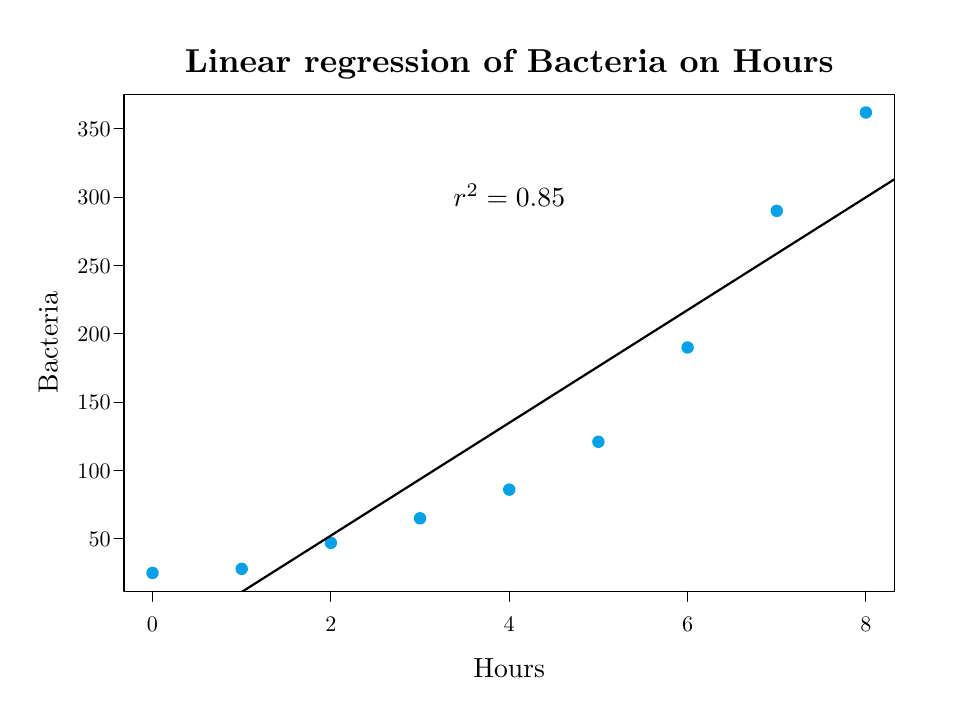
\begin{tikzpicture}[x=1pt,y=1pt]
\definecolor{fillColor}{RGB}{255,255,255}
\path[use as bounding box,fill=fillColor,fill opacity=0.00] (0,0) rectangle (325.21,238.49);
\begin{scope}
\path[clip] ( 34.80, 34.80) rectangle (313.21,214.49);
\definecolor{fillColor}{RGB}{5,161,230}

\path[fill=fillColor] ( 45.11, 41.46) circle (  2.25);

\path[fill=fillColor] ( 77.34, 42.94) circle (  2.25);

\path[fill=fillColor] (109.56, 52.32) circle (  2.25);

\path[fill=fillColor] (141.78, 61.20) circle (  2.25);

\path[fill=fillColor] (174.01, 71.57) circle (  2.25);

\path[fill=fillColor] (206.23, 88.85) circle (  2.25);

\path[fill=fillColor] (238.46,122.92) circle (  2.25);

\path[fill=fillColor] (270.68,172.29) circle (  2.25);

\path[fill=fillColor] (302.90,207.84) circle (  2.25);
\end{scope}
\begin{scope}
\path[clip] (  0.00,  0.00) rectangle (325.21,238.49);
\definecolor{drawColor}{RGB}{0,0,0}

\path[draw=drawColor,line width= 0.4pt,line join=round,line cap=round] ( 45.11, 34.80) -- (302.90, 34.80);

\path[draw=drawColor,line width= 0.4pt,line join=round,line cap=round] ( 45.11, 34.80) -- ( 45.11, 31.21);

\path[draw=drawColor,line width= 0.4pt,line join=round,line cap=round] (109.56, 34.80) -- (109.56, 31.21);

\path[draw=drawColor,line width= 0.4pt,line join=round,line cap=round] (174.01, 34.80) -- (174.01, 31.21);

\path[draw=drawColor,line width= 0.4pt,line join=round,line cap=round] (238.46, 34.80) -- (238.46, 31.21);

\path[draw=drawColor,line width= 0.4pt,line join=round,line cap=round] (302.90, 34.80) -- (302.90, 31.21);

\node[text=drawColor,anchor=base,inner sep=0pt, outer sep=0pt, scale=  0.80] at ( 45.11, 20.40) {0};

\node[text=drawColor,anchor=base,inner sep=0pt, outer sep=0pt, scale=  0.80] at (109.56, 20.40) {2};

\node[text=drawColor,anchor=base,inner sep=0pt, outer sep=0pt, scale=  0.80] at (174.01, 20.40) {4};

\node[text=drawColor,anchor=base,inner sep=0pt, outer sep=0pt, scale=  0.80] at (238.46, 20.40) {6};

\node[text=drawColor,anchor=base,inner sep=0pt, outer sep=0pt, scale=  0.80] at (302.90, 20.40) {8};

\path[draw=drawColor,line width= 0.4pt,line join=round,line cap=round] ( 34.80, 53.80) -- ( 34.80,201.91);

\path[draw=drawColor,line width= 0.4pt,line join=round,line cap=round] ( 34.80, 53.80) -- ( 31.21, 53.80);

\path[draw=drawColor,line width= 0.4pt,line join=round,line cap=round] ( 34.80, 78.48) -- ( 31.21, 78.48);

\path[draw=drawColor,line width= 0.4pt,line join=round,line cap=round] ( 34.80,103.17) -- ( 31.21,103.17);

\path[draw=drawColor,line width= 0.4pt,line join=round,line cap=round] ( 34.80,127.85) -- ( 31.21,127.85);

\path[draw=drawColor,line width= 0.4pt,line join=round,line cap=round] ( 34.80,152.54) -- ( 31.21,152.54);

\path[draw=drawColor,line width= 0.4pt,line join=round,line cap=round] ( 34.80,177.23) -- ( 31.21,177.23);

\path[draw=drawColor,line width= 0.4pt,line join=round,line cap=round] ( 34.80,201.91) -- ( 31.21,201.91);

\node[text=drawColor,anchor=base east,inner sep=0pt, outer sep=0pt, scale=  0.80] at ( 30.00, 51.04) {50};

\node[text=drawColor,anchor=base east,inner sep=0pt, outer sep=0pt, scale=  0.80] at ( 30.00, 75.73) {100};

\node[text=drawColor,anchor=base east,inner sep=0pt, outer sep=0pt, scale=  0.80] at ( 30.00,100.41) {150};

\node[text=drawColor,anchor=base east,inner sep=0pt, outer sep=0pt, scale=  0.80] at ( 30.00,125.10) {200};

\node[text=drawColor,anchor=base east,inner sep=0pt, outer sep=0pt, scale=  0.80] at ( 30.00,149.78) {250};

\node[text=drawColor,anchor=base east,inner sep=0pt, outer sep=0pt, scale=  0.80] at ( 30.00,174.47) {300};

\node[text=drawColor,anchor=base east,inner sep=0pt, outer sep=0pt, scale=  0.80] at ( 30.00,199.16) {350};

\path[draw=drawColor,line width= 0.4pt,line join=round,line cap=round] ( 34.80, 34.80) --
	(313.21, 34.80) --
	(313.21,214.49) --
	( 34.80,214.49) --
	( 34.80, 34.80);
\end{scope}
\begin{scope}
\path[clip] (  0.00,  0.00) rectangle (325.21,238.49);
\definecolor{drawColor}{RGB}{0,0,0}

\node[text=drawColor,anchor=base,inner sep=0pt, outer sep=0pt, scale=  1.20] at (174.01,222.30) {\bfseries Linear regression of Bacteria on Hours};

\node[text=drawColor,anchor=base,inner sep=0pt, outer sep=0pt, scale=  1.00] at (174.01,  3.60) {Hours};

\node[text=drawColor,rotate= 90.00,anchor=base,inner sep=0pt, outer sep=0pt, scale=  1.00] at ( 10.80,124.65) {Bacteria};
\end{scope}
\begin{scope}
\path[clip] ( 34.80, 34.80) rectangle (313.21,214.49);
\definecolor{drawColor}{RGB}{0,0,0}

\path[draw=drawColor,line width= 0.8pt,line join=round,line cap=round] ( 34.80,  7.69) -- (313.21,183.72);

\node[text=drawColor,anchor=base,inner sep=0pt, outer sep=0pt, scale=  1.00] at (174.01,173.76) {$r^2=0.85$};
\end{scope}
\end{tikzpicture}
